\documentclass[10pt]{article}
\textwidth= 5.00in
\textheight= 7.4in
\topmargin = 30pt
\evensidemargin=0pt
\oddsidemargin=55pt
\headsep=17pt
\parskip=.5pt
\parindent=12pt
\font\smallit=cmti10
\font\smalltt=cmtt10
\font\smallrm=cmr9

\usepackage{amssymb,latexsym,amsmath,epsfig,amsthm, graphicx, centernot}

\makeatletter

\renewcommand\section{\@startsection {section}{1}{\z@}
{-30pt \@plus -1ex \@minus -.2ex}
{2.3ex \@plus.2ex}
{\normalfont\normalsize\bfseries\boldmath}}

\renewcommand\subsection{\@startsection{subsection}{2}{\z@}
{-3.25ex\@plus -1ex \@minus -.2ex}
{1.5ex \@plus .2ex}
{\normalfont\normalsize\bfseries\boldmath}}

\renewcommand{\@seccntformat}[1]{\csname the#1\endcsname. }

\newcommand\blfootnote[1]{
\begingroup
\renewcommand\thefootnote{}\footnote{#1}
\addtocounter{footnote}{-1}
\endgroup
}

\makeatother

\newtheorem{theorem}{Theorem}
\newtheorem{lemma}{Lemma}
\newtheorem{proposition}{Proposition}
\newtheorem{corollary}{Corollary}

\theoremstyle{definition}
\newtheorem{definition}{Definition}
\newtheorem{conjecture}{Conjecture}
\newtheorem{remark}{Remark}
\newtheorem{example}{Example}

\begin{document}

\begin{center}
\uppercase{\bf \boldmath Vector Recurrence Hailstone Sequence}
\vskip 20pt
{\bf J. Collins}\\
{\smallit Department of Mathematics, Grove City College, Grove City, PA, USA}\\
{\tt CollinsJD23@gcc.edu}\\
\end{center}

\centerline{\bf Abstract}
\noindent
We explore a vector sequence, $V$, generated from the initial vector $v_0$ and operator $T_n$ where this operator is defined in part by the Hailstone sequence and exponential decay. Emerging properties of the vectors within $V$ are parity, multiple memory cells, non-monotonic behavior, and cycles.

\pagestyle{myheadings}
\thispagestyle{empty}
\baselineskip=12.875pt
\vskip 30pt

\section{Introduction}

*Background/why this matters and is related to things*

\section{Basic Definitions}

We first define some basic terminology outlining the object(s) of exploration.

\begin{definition}
    Let $v_n$ be an $n$-dimensional integer vector.
\end{definition}

\begin{definition}
    Let the vector sequence is $V=\{v_0,v_1,...,v_n\}$.
\end{definition}

\begin{definition}
    We define the following recursive definition where $T_k:\mathbb{N}^n \xrightarrow{} \mathbb{N}^{n+1}$ and $S(\cdot)$ is some sequence rule applied to $\cdot$,
    \begin{center}
        $v_0=(x_0)$
    
        $v_{n+1}=T_k(v_n)=(\lfloor x_0/k \rfloor, \lfloor x_1/k \rfloor,...,\lfloor x_n/k \rfloor, S(\sum_i \lfloor x_i/k \rfloor))$
    \end{center}
\end{definition}

We will look at different $k$ values and $S$ rules.

\section{Hailstone Sequence}

See the following GitHub repository to find the custom GUI made for organizing information from this section: 

https://github.com/greenTortle/vector\_sequence\_GUI/blob/main/balancing\_k.py

In this section we will consider $S$ to be the rules of the Hailstone Sequence. In doing so we have noticed 3 vector sequence patterns: zeroing, cycling, and growing.

\begin{definition}
    We say zeroing is the process of $v_n \xrightarrow{} (0,...,0)$ as $n \xrightarrow{} \infty$.
\end{definition}

\begin{definition}
    We say cycling is the occurrence of $v_n=v_{n+k}$ for some $k>0$ .
\end{definition}

\begin{definition}
    We say growing is a sequence which neither zeroes nor cycles. 
\end{definition}

Experimentally looking at a range of $k$ values has shows tendencies of $V$; these results have seem to be independent of $x_0$ and checked up to $x_0=2000$. Based on this we can create a piecewise relationship of $V$ in terms of $k$ and some notation,

\begin{definition}
    We say $G_\#$ is the number of growing vector sequences in $V$.
\end{definition}

\begin{definition}
    We say $Z_\#$ is the number of zeroing vector sequences in $V$.
\end{definition}

\begin{definition}
    We say $C_\#$ is the number of cycling vector sequences in $V$.
\end{definition}

\begin{definition}
    We say $\Sigma_\#$ is the total number of vector sequences in $V$.
\end{definition}

With these definitions we can experimentally say a tendency of $V$ is,

\[ 
\begin{cases}
Z_\# > G_\# & \text{if } k \ge 2.5 \\
G_\# \approx{} Z_\# & \text{if } 2.35 < k < 2.5 \\
G_\# > Z_\# & \text{if } k < 2.35
\end{cases}
\]

\begin{figure}[h]
    \centering
    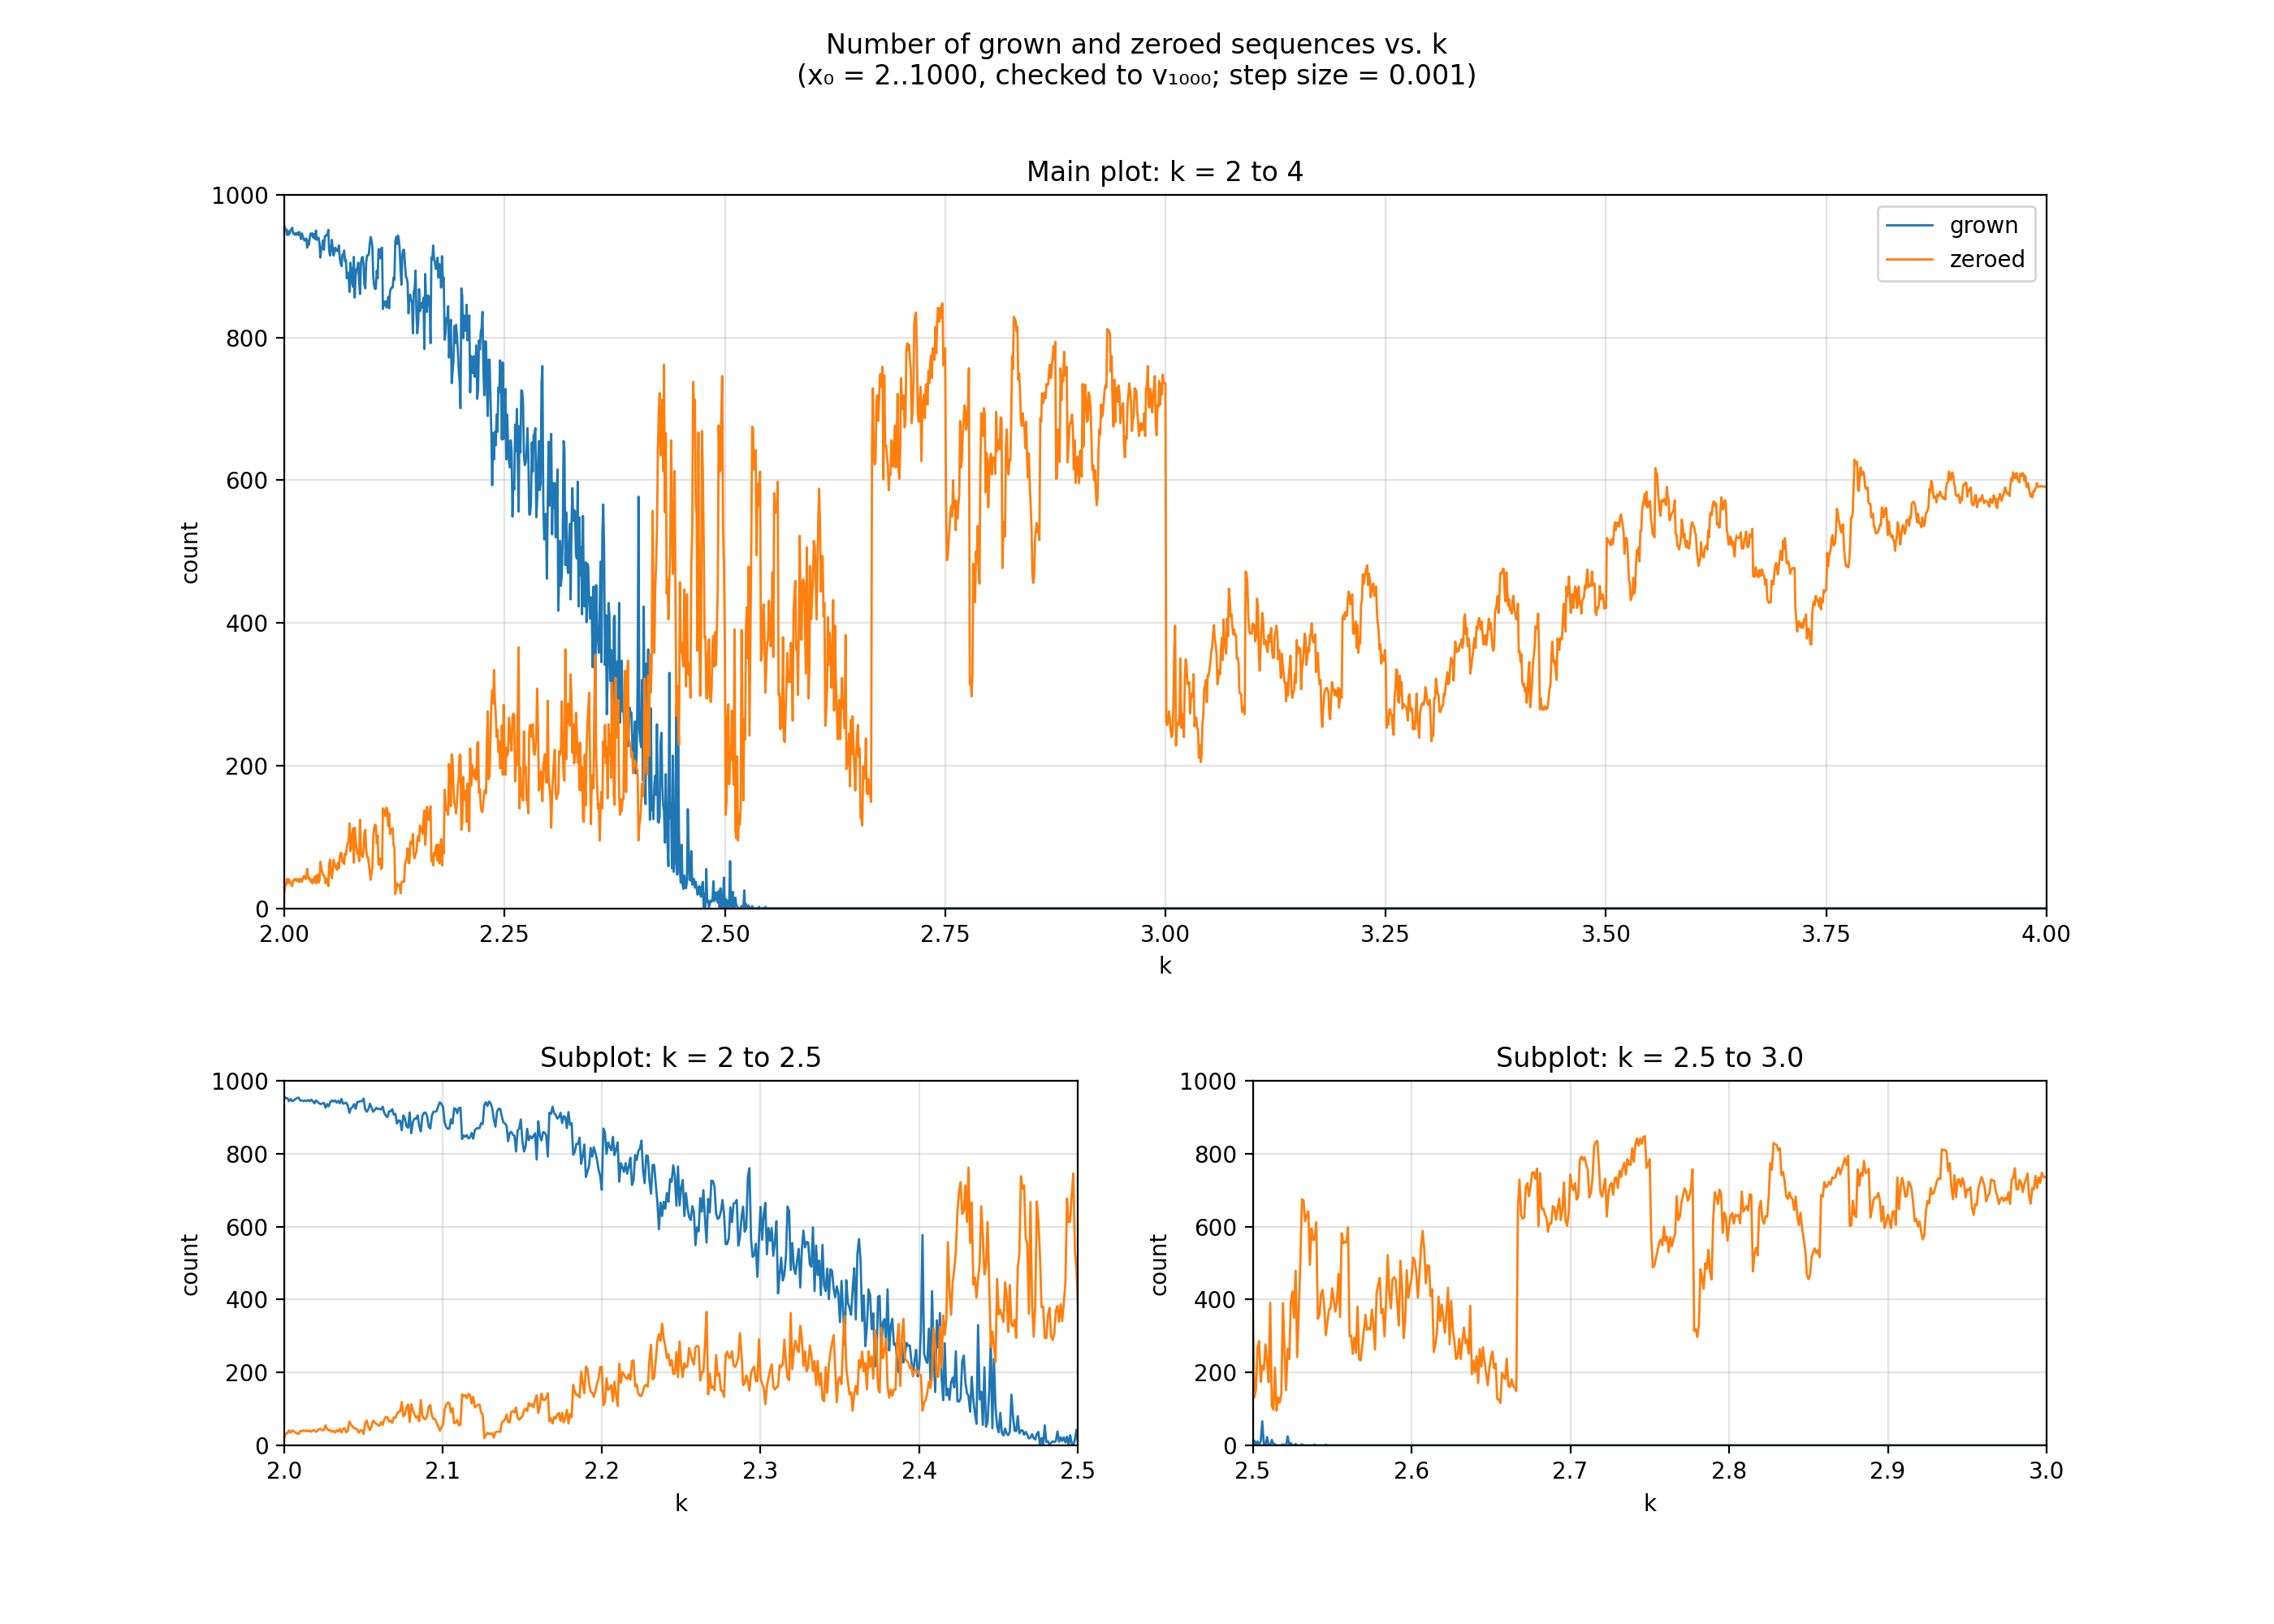
\includegraphics[width=1\textwidth]{k_grown_zeroed_multiplot_2_4.png}
    \label{fig:myfigure}
\end{figure}

Beyond $V$, other experimental patterns are...

\[ 
G_\# \approx{}
\begin{cases}
0 & \text{if } k \ge 2.5 \\
5050-2500k & \text{if } 2.3 < k < 2.5 \\
1000 & \text{if } k < 2.3
\end{cases}
\]

\[ 
Z_\# \approx{}
\begin{cases}
1000 & \text{if } k \ge 4 \\
? & \text{if } 2 < k < 2.5 \\
\approx{} 0 & \text{if } k < 2
\end{cases}
\]


From the graphs below, it appears that within $2<k<4$, three sections of $Z_\#$ values stand out: $2<k<2.666..., 2.666...<k<3,$ and $3<k<4$. In the first region the average change per increment of $k$ seems to be larger and ends with a large jump at $k=2.666$. In the second region, higher $Z_\#$ values are generally seen until $k=3$ and there is a large jump in $Z_\#$ into the third region. Here $Z_\#$ generally trends from 300 to 600 until at $k>4$ it jumps to 1000.

At $k=2.666..., 2.777..., \text{ and } 3$ there are large jumps in $Z_\#$, but these also exist at $k\approx{} 2.4690026954, 2.47058$ and others, although they do not have a nice closed form.

\end{document}